\section{Surrogate Models}
%-----------------------------------------------------------------------
%-----------------------------------------------------------------------
\begin{frame}[c]{Characteristics we Require our Surrogate Models to Have}

\begin{columns}[T] % align columns
\begin{column}{.48\textwidth}
    \begin{block}{Mandatory}
    \begin{itemize}
    	\item Regression model
    	\item Uncertainty estimates
    	\item Accurate predictions
    \end{itemize}
    \end{block}
    
\pause
        \begin{block}{Depending on the application}
        \begin{itemize}
        	\item Cheap-to-train
        	\item Scales with the complexity of the data
        	\note[item]{(number of features and observations)}
        	\item Can handle different types of inputs
        	\note[item]{(categorical and continuous)}
        \end{itemize}
        \end{block}
    
\end{column}%

\hfill%

\begin{column}{.48\textwidth}

%\only<1-1>{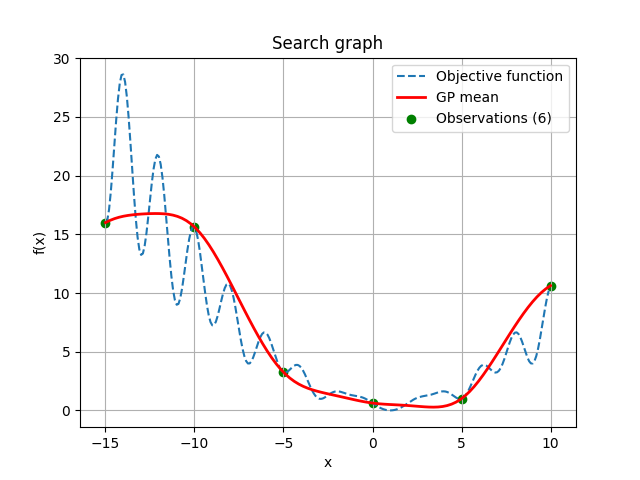
\includegraphics[width=1.\textwidth]{images/bo_loop_overview/03_mean.png}}
%\only<2-6>{
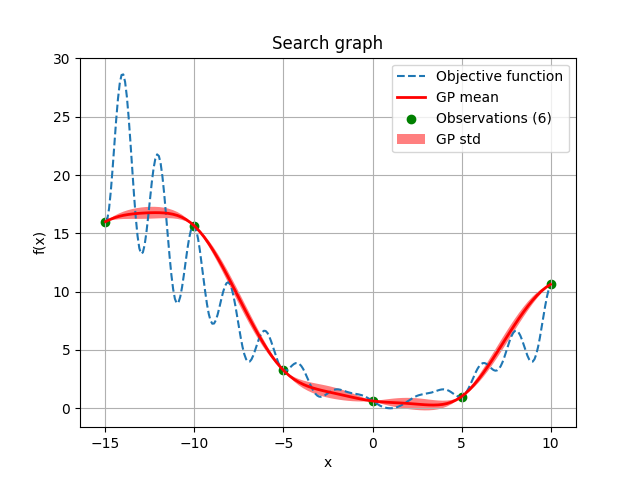
\includegraphics[width=1.\textwidth]{images/bo_loop_overview/04_std.png}
%}

\end{column}%
\end{columns}

\end{frame}
%-----------------------------------------------------------------------

%-----------------------------------------------------------------------
%-----------------------------------------------------------------------
\begin{frame}[c]{Surrogate Models we Will Discuss}

\begin{columns}[T] % align columns
\begin{column}{.48\textwidth}
\begin{itemize}
	\item<1-3> Gaussian Processes \note[item]{(quite common)}
	\item<2-3> Random Forests \note[item]{(our default choice)}
	\item<3-3> Bayesian Neural Networks \note[item]{(recent trend)}
\end{itemize}
\end{column}%

\hfill%

\begin{column}{.48\textwidth}
\only<1-1>{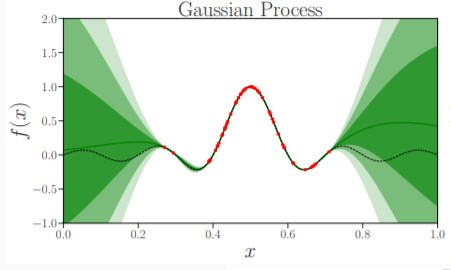
\includegraphics[width=1.\textwidth]{images/surrogate_models/uncertainty_gp.jpg}}
\only<2-2>{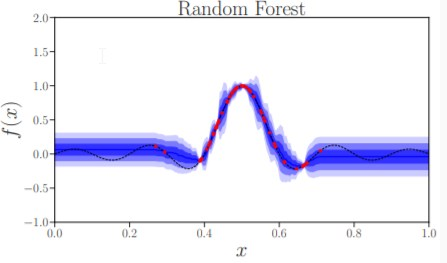
\includegraphics[width=1.\textwidth]{images/surrogate_models/uncertainty_forest.jpg}}
\only<3-3>{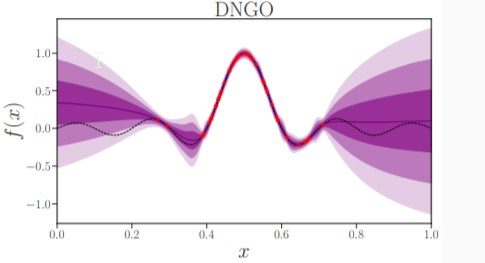
\includegraphics[width=1.\textwidth]{images/surrogate_models/uncertainty_dngo.jpg}}
\end{column}%
\end{columns}

\source{A. Klein: Introduction Automated Machine Learning}

\comment{adjust those plots
FH: best to have plots stay on the slide, e.g., next to each other.}

\end{frame}
%-----------------------------------------------------------------------

%-----------------------------------------------------------------------
%-----------------------------------------------------------------------
\begin{frame}[c]{Gaussian Processes - reminder}

\begin{columns}[T] % align columns
\begin{column}{.48\textwidth}

    \begin{block}{Advantages}
    \begin{itemize}
    	\item Smooth and reliable uncertainty estimates 
		\item Sample efficiency
    	\item We can encode expert knowledge about the design space in the kernel 
    \end{itemize}
    \end{block}
\end{column}%

\hfill%
\pause

\begin{column}{.48\textwidth}
    \begin{block}{Disadvantages}
    \begin{itemize}
    	\item We have to define a good kernel for each application 
    	\note[item]{(if we don't optimize small-dimensional, continuous functions)}
    	\item Cost scales cubically with the number of observations 
    	\note[item]{(because of inverting the kernel)}
    	\item Not easily applicable in discrete or conditional spaces 
    	\item Sensitive to its own hyperparameters
    \end{itemize}
\end{block}

\end{column}
\end{columns}

\note[item]{
	\begin{itemize}
		 \item e.g., special kernels for categorical hyperparameters and\\ conditional dependencies
	\end{itemize}
}
	
\note[item]{
    \begin{itemize}
    	\item to address this issue, there are sparse GPs\\ \lit{Snelson and Ghahramani. 2005}
    \end{itemize}
}

\end{frame}
%-----------------------------------------------------------------------

%-----------------------------------------------------------------------
%-----------------------------------------------------------------------
%\begin{frame}[c]{Gaussian Processes - reminder}
%
%\begin{itemize}
%    \item<1-3> The prior is a GP with constant mean and variance; draws are jointly Gaussian
%    \item<2-3> The kernel (covariance) function $K$ tells us how correlated the function values at two points are
%    \item<3-3> The posterior is also a GP, with predictive distribution:
 %   \begin{equation*}
 %        P(\func_{\bocount+1} \vert \dataset_{1:\bocount}, \conf_{\bocount+1}) =  \mathcal{N}(\mean_{\bocount}(\conf_{\bocount+1}), \variance_{\bocount}(\conf_{\bocount+1}))
 %   \end{equation*}
 %   \begin{equation*}
 %       \mean_{\bocount}(\conf_{\bocount+1}) = \bm{k}^{T} \bm{K}^{-1} \bm{\func_{1:\bocount}}
 %   \end{equation*}
 %   \begin{equation*}
 %       \variance_{\bocount}(\conf_{\bocount+1}) = k(\conf_{\bocount+1}, \conf_{\bocount+1}) - \bm{k}^{T} \bm{K}^{-1} \bm{k}
 %   \end{equation*}
%\end{itemize}
%
%\note[item]{for the review of GPs - Rasmussen and Williams}
%
%\end{frame}
%-----------------------------------------------------------------------
 
%-----------------------------------------------------------------------
%-----------------------------------------------------------------------
\begin{frame}[c]{Surrogate Models: GPs - kernel hyperparameters}

\begin{itemize}
    \item After choosing the kernel, we must also manage the hyperparameters that govern its behaviour, as well as that of the mean function.  \pause
    \item For our problems of interest, typically we have $D + 3$ GPs hyperparameters:  
    \begin{itemize}
        \item $D$ length scales $\theta_{1:D}$, 
        \item the covariance amplitude $\theta_{0}$, 
        \item the observation noise $\noise$, 
        \item a constant mean $\mean$. 
    \end{itemize}
\end{itemize}

\end{frame}
%-----------------------------------------------------------------------

%-----------------------------------------------------------------------
%-----------------------------------------------------------------------
\begin{frame}[c]{Surrogate Models: GPs - kernel hyperparameters}

\begin{columns}[T] % align columns
\begin{column}{.58\textwidth}
\begin{itemize}
    \item We can use Maximum A Posteriori (MAP) or Maximum Likelihood Estimation (MLE) to sample hyperparameters 
    \item However, it is more realistic not to assume that hyperparameters distribution can be represented by a single point
\end{itemize}
\end{column}%

\hfill%

\begin{column}{.38\textwidth}
\end{column}%
\end{columns}

%\source{Snoek et al. 2015}
\end{frame}
%-----------------------------------------------------------------------

%-----------------------------------------------------------------------
%-----------------------------------------------------------------------
\begin{frame}[c]{Surrogate Models: GPs - kernel hyperparameters}

\begin{columns}[T] % align columns
\begin{column}{.58\textwidth}
\begin{itemize}
    \item<1-4> Markov-Chain Monte-Carlo (MCMC) drops this assumption and samples hyperparameters from a distribution proportional to their probability, given the data and prior assumptions
    \item<2-4> Marginalize over hyperparameters and compute integrated acquisition function:
        \begin{equation*}
        \begin{aligned}
            \hat{\acq} ( \conf; \left \{ \bonextsample, \bonextobs \right \} ) = \int \acq ( \conf; \left \{ \bonextsample, \bonextobs \right \}, \theta ) \\ 
            p(\theta  \rvert \left \{ \bonextsample, \bonextobs \right \}^{\bobudget}_{\bocount=1} )d\theta
        \end{aligned}
        \end{equation*}
    \item<3-4> MCMC is more computationally expensive than gradient based optimization
    \item<4-4>The acquisition function must now be calculated more than just once
\end{itemize}
\end{column}%

\hfill%

\begin{column}{.38\textwidth}
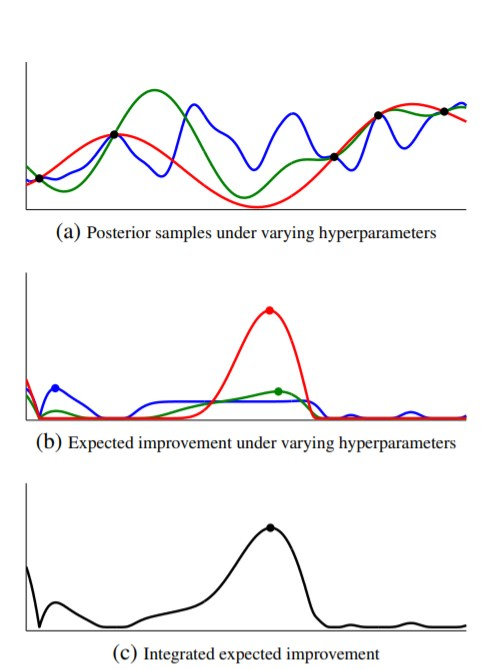
\includegraphics[width=0.9\textwidth]{images/surrogate_models/kernel_hp_mcmc.jpg}
\end{column}%
\end{columns}

\source{Snoek et al. 2015}
\end{frame}
%-----------------------------------------------------------------------

%-----------------------------------------------------------------------
%-----------------------------------------------------------------------
\begin{frame}[c]{Surrogate Models: Random Forests}

\begin{columns}[T] % align columns
\begin{column}{.48\textwidth}


\begin{block}{Train}
\begin{itemize}
	\item $n$ regression trees
	\item Subsampled training data for each tree (with bootstrapping)
	\item Each tree gives us a possible explanation for the observations
\end{itemize}
\end{block}

\pause
    \begin{block}{Predict}
    \begin{itemize}
    	\item Obtain prediction of each tree
    	\item Aggregate predictions (e.g., average)
    	\item Uncertainty of predictions: stdev across tree predictions
    \end{itemize}
    \end{block}

\end{column}%

\note[item]{Uncertainty in the leaves is dropped}

\hfill%

\begin{column}{.48\textwidth}
    \centering
    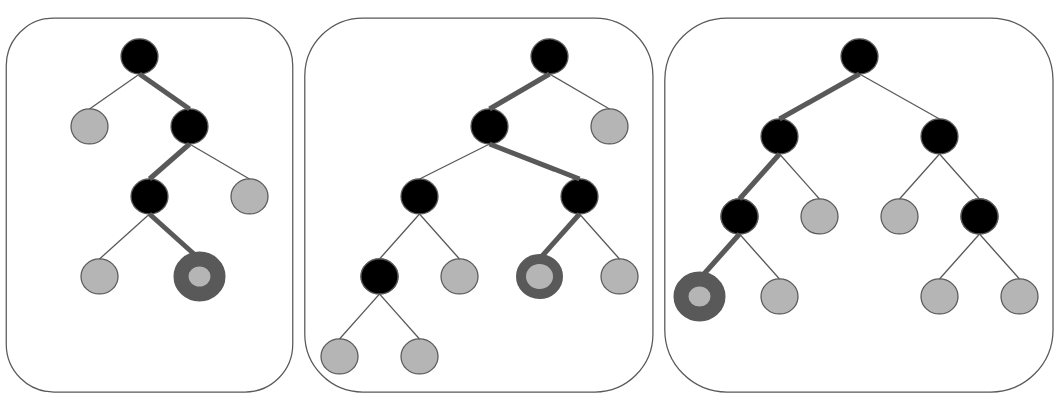
\includegraphics[width=0.8\textwidth]{images/surrogate_models/random_forest_pic}
\end{column}
\end{columns}

\end{frame}
%-----------------------------------------------------------------------

%-----------------------------------------------------------------------
%-----------------------------------------------------------------------
\begin{frame}[c]{Surrogate Models: Random Forests - hyperparameters}

\begin{columns}
	\column{0.5\textwidth}
	\centering
	w bootstrapping and\\ w/o random splits
	
	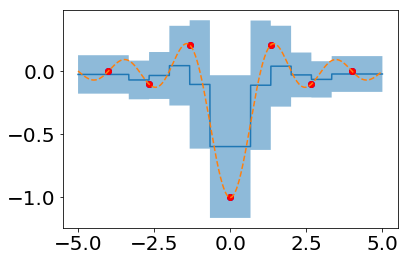
\includegraphics[width=0.6\textwidth]{images/surrogate_models/rf_boot_middle_split.png}
	
	
	w bootstrapping and\\ w/ random splits
	
	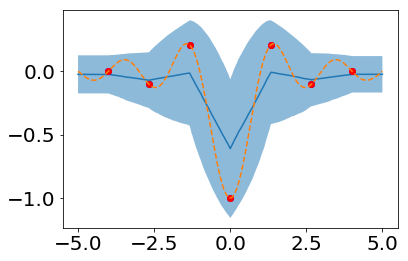
\includegraphics[width=0.6\textwidth]{images/surrogate_models/rf_boot_rand_split.png}

	\column{0.5\textwidth}
	\centering
	w/o bootstrapping and\\ w/o random splits
	
	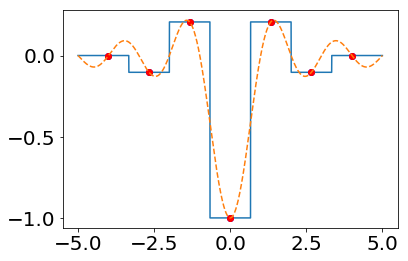
\includegraphics[width=0.6\textwidth]{images/surrogate_models/rf_noboot_middle_split.png}
	
	w/o bootstrapping and\\ w/ random splits
	
	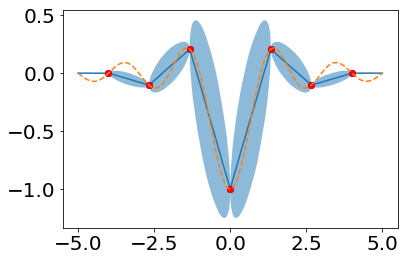
\includegraphics[width=0.6\textwidth]{images/surrogate_models/rf_noboot_rand_split.png}
	
\end{columns}

\end{frame}
%-----------------------------------------------------------------------

%-----------------------------------------------------------------------
%-----------------------------------------------------------------------
\begin{frame}[c]{Surrogate Models: Random Forests - summary}


\begin{columns}[T] % align columns
\begin{column}{.48\textwidth}

    \begin{block}{Advantages}
    \begin{itemize}
        \item Cheap to train 
        \item Scales well with \#observations: 
        \begin{itemize}
        	\item Worst-case complexity for $T$ tress with $n$ data points of dimensionality $p$: $\mathcal O(T\cdot p \cdot n^2 \log{n})$. 
        \end{itemize}
        \item Training can be parallelized 
        \item Can easily handle conditional, categorical, continuous and discrete spaces 
        \item Quite robust against its own hyperparameters
    \end{itemize}
    \end{block}
\end{column}%

\hfill%
\pause

\begin{column}{.48\textwidth}
    \begin{block}{Disadvantages}
    \begin{itemize}
        \item Poor uncertainty estimates 
        \item Poor extrapolation (constant) 
    	\item Priors cannot be incorporated easily 
    \end{itemize}
    \end{block}

\end{column}
\end{columns}

\end{frame}
%-----------------------------------------------------------------------

%-----------------------------------------------------------------------
%-----------------------------------------------------------------------
\begin{frame}[c]{Surrogate Models: Bayesian Neural Networks - Idea}

\begin{itemize}
    \item Deal with all sources of parameter uncertainty: \pause
    \begin{itemize}
        \item More than one weight vector can explain the observed data 
        \item Take into account all possible explanations 
    \end{itemize}

\centering
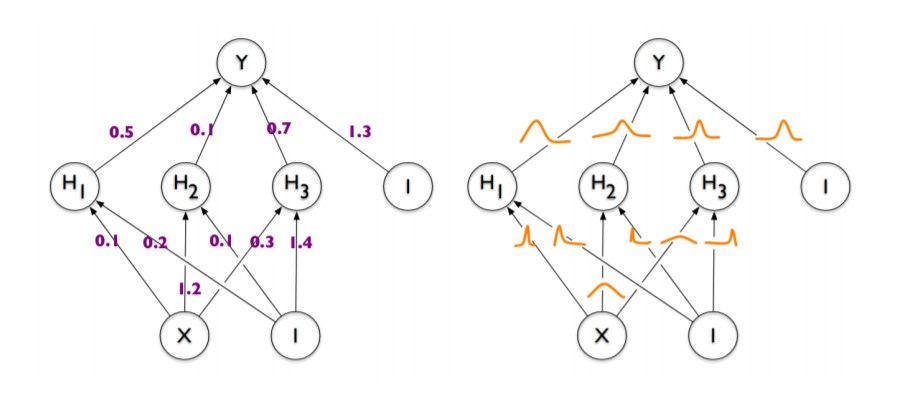
\includegraphics[width=0.6\textwidth]{images/surrogate_models/bnn.jpg}

\end{itemize}

\source{Blundell et al.: Weight Uncertainty in Neural Networks}

\end{frame}
%-----------------------------------------------------------------------

%-----------------------------------------------------------------------
%-----------------------------------------------------------------------
\begin{frame}[c]{Surrogate Models: Bayesian Neural Networks - Idea}

\begin{itemize}
    \item Deal with all sources of parameter uncertainty
    \item If possible, one would also deal with uncertainty about the network architecture
     \begin{itemize}
        \item For every architecture, one would still want to be Bayesian about its weights... 
        \item Nobody is really Bayesian about architectures these days 
        \item This has been too expensive; but that may change with efficient
gradient-based architecture search methods...
    \end{itemize}
\end{itemize}

\end{frame}
%-----------------------------------------------------------------------


%-----------------------------------------------------------------------
%-----------------------------------------------------------------------
\begin{frame}[c]{Surrogate Models: NNs for Bayesian optimization}

\begin{itemize}
	\item NNs work well given large data sets
	\item In Bayesian optimization, we (often) have few data points
	\item Nevertheless, we can use NNs for BO when we handle uncertainty well\pause
	\bigskip
	\item Overview of examples using NNs for BO:
	\begin{itemize}
	    \item Snoek et al.: Scalable Bayesian Optimization Using Deep Neural Networks
	    \item Springenberg et al.: Bayesian Optimization with Robust Bayesian Neural Networks
        \item Schilling et al.: Hyperparameter Optimization with Factorized Multilayer Perceptrons
        \item Perrone et al.: Scalable Hyperparameter Transfer Learning
        \item Hern\'andez-Lobato et al.: Parallel and Distributed Thompson Sampling for Large-scale Accelerated Exploration of Chemical Space
	\end{itemize}
\end{itemize}

\end{frame}
%-----------------------------------------------------------------------

%-----------------------------------------------------------------------
%-----------------------------------------------------------------------
\begin{frame}[c]{Surrogate Models: the Bayesian Neural Networks - DNGO}

\begin{itemize}
    \item Fit a standard neural network to the data 
    \item Use the representation in the last hidden layer as basis \\ functions $\phi(x)$ of the input $x$ 
    \item Use Bayesian linear regression for the output layer \pause
    \begin{itemize}
        \item The last layer is linear in its parameters $\theta$  
        \item Therefore, the Bayesian linear regression formulas work directly 
        \item Feasible in closed form, in time $O(N d^3)$, \\ where $N$ is the number of data points and $d$ is the number of \\ hidden units in the last layer 
    \end{itemize}
    
\end{itemize}

\end{frame}
%-----------------------------------------------------------------------

%-----------------------------------------------------------------------
%-----------------------------------------------------------------------
\begin{frame}[c]{Surrogate Models: DNGO - summary}


\begin{columns}[T] % align columns
\begin{column}{.48\textwidth}

    \begin{block}{Advantages}
    \begin{itemize}
        \item Scales linearly with \#observations 
        \item Given enough network samples obtain nice and smooth uncertainty estimates 
        \item Can handle categorical, continuous and discrete spaces
    \end{itemize}
    \end{block}
\end{column}%

\hfill%
\pause

\begin{column}{.48\textwidth}
    \begin{block}{Disadvantages}
    \begin{itemize}
        \item Poor uncertainty estimates 
        \item Many meta-design decisions 
    	\item No robust off-the-shelf implementation 
    	\item Usually needs more data than Gaussian processes
    \end{itemize}
    \end{block}

\end{column}
\end{columns}

\end{frame}
%-----------------------------------------------------------------------
